\chapter{Proses Bisnis dan Pengumpulan Data Fisik}

\section{Proses Bisnis}
Dalam melakukan penganalisaan pada rancangan database mengenai pembuatan passpor, maka perlu di ketahui alur maupun proses dalam rancangan tersebut atau disebut juga sebagai proses bisnis. maka prosesnya sebagai berikut :
\begin{enumerate}
	\item Pemohon Datang langsung ke kantor imigrasi setempat atau terdekat serta membawa dokumen dan alat tulis yang dimasukan kedalam map
	\item Jangan lupa menggunakan pakaian rapi. Disarankan memakai baju selain warna putih (karena sewaktu berfoto, backgroundnya putih)
	\item Berikan kode booking atau foto QR Barcode pada petugas layanan, lalu ia akan mengscan QR Barcode dalam bentuk cetak berisi nomor urut
	\item Petugas akan mengecek atau memeriksa kelengkapan dokumen lalu memberi formulis data diri
    \item Isi formulir data diri dengan benar sesuai dengan petujuk yang ada pada formulir tersebut
    \item Saat dipanggil, berikan smeua dokumen kepada petugas
    \item kumdian akan ada sesi Wawancara singkat oleh petugas
    \item sesi Pemindaian sidik jari dan sesi foto oleh petugas
    \item selanjutnya akan ada Instruksi pembayaran biaya pembuatan
\end{enumerate}
\subsection{Syarat-syarat pembuatan Passpor}
\begin{enumerate}
\item E-ktp asli beserta fotokopinya
\item Kartu keluarga asli beserta fotokopinya
\item Akta kelahiran, ijazah(SD/SMP/SMA), surat/buku nikah, atau surat Baptis asli beserta fotokopinya. Untuk dokumen ini, hanya perlu, memilih, salah satunya saja, misalnya hanya akta kelahiran. Namun,pastikan pada dokumen terdapat informasi mengenai nama,tempat dan tanggal lahir, serta nama orang tua
\item Siapakan materei 6000

\section{Pengumpulan Data Fisik}
Data fisik sangat dibutuhkan untuk membuat passpor adapun Bukti fisiknya sebagai berikut :  
\end{enumerate}
\begin{enumerate}

	\item Kartu Keluarga Keluarga Pertama
	\begin{figure}[H]
		\centering
		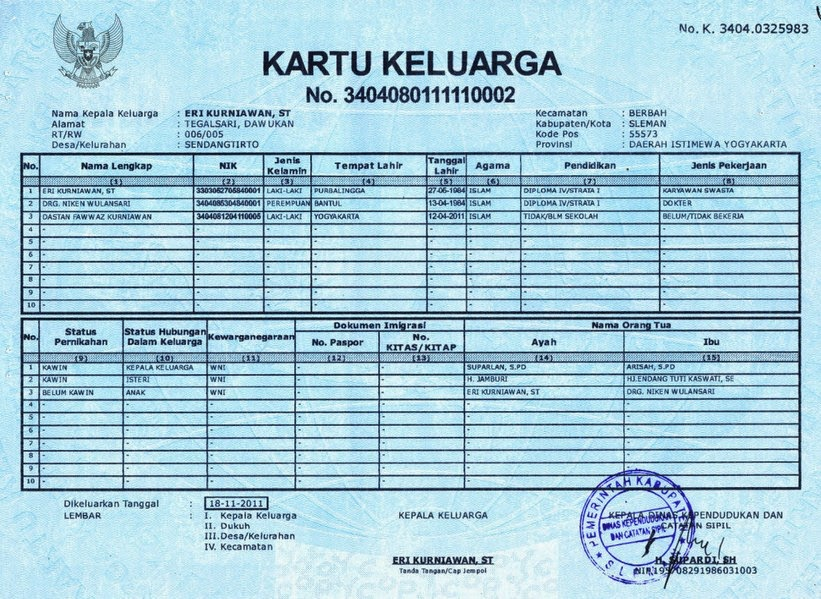
\includegraphics[width=12cm]{figures/kk.jpg}
		\caption{Kartu Keluarga.}	
	\end{figure}

	\item Akta Kelahiran
	\begin{figure}[H]
		\centering
		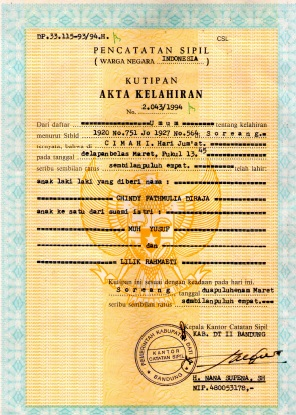
\includegraphics[width=12cm]{figures/akte.jpg}
		\caption{Akta Kelahiran.}	
	\end{figure}

	\item Formulir Paspor
	\begin{figure}[H]
		\centering
		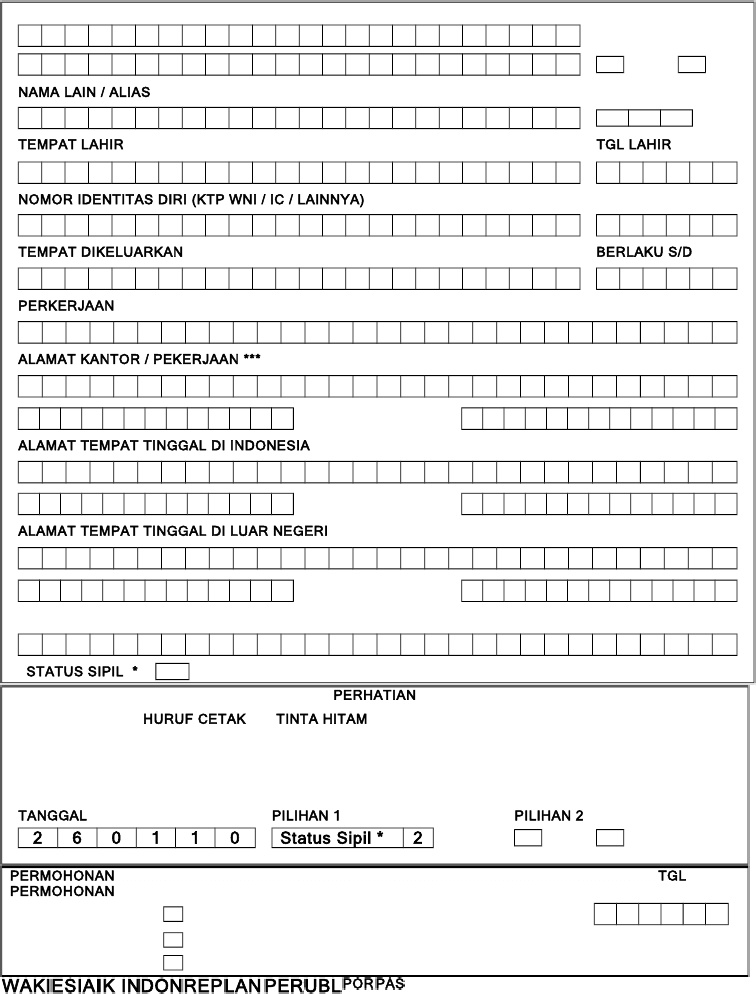
\includegraphics[width=12cm]{figures/formulirpaspor.jpg}
		\caption{Formulir Data Paspor}	
	\end{figure}

	\item Surat Baptis
	\begin{figure}[H]
		\centering
		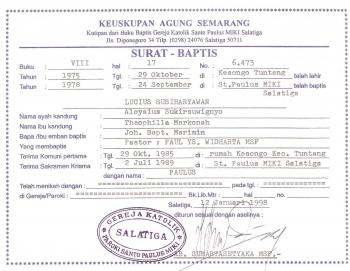
\includegraphics[width=12cm]{figures/suratbaptis.jpg}
		\caption{Surat Baptis}	
	\end{figure}

	\item e-KTP
	\begin{figure}[H]
		\centering
		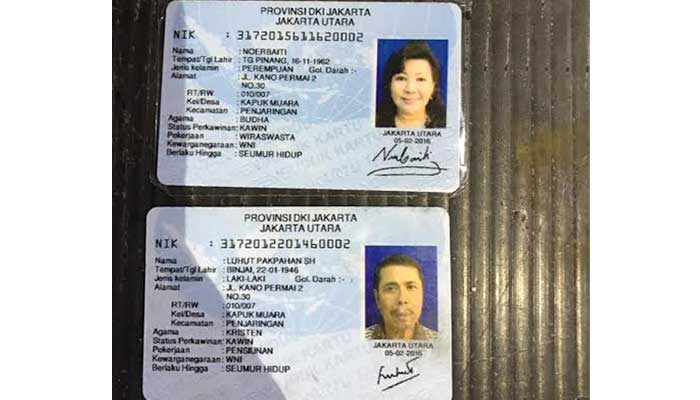
\includegraphics[width=12cm]{figures/ktp.jpg}
		\caption{e-KTP.}	
	\end{figure}

	\item Buku Nikah
	\begin{figure}[H]
		\centering
		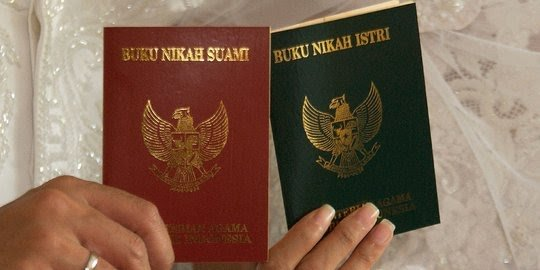
\includegraphics[width=12cm]{figures/bukunikah.jpg}
		\caption{Buku Nikah.}	
	\end{figure}
\end{enumerate}